\documentclass[UTF8,fontset=none,aspectratio=169,10pt]{beamer}
\usepackage{ads-beamer-theme}

\title{高级分布式系统}
\subtitle{第七讲：消息序、同步通信与组播}
\author{陈鹏飞\quad 计算机学院}
\institute{中山大学}
\date{2025--2026 学年}

\begin{document}

\begin{frame}[plain]
\begin{tikzpicture}[remember picture,overlay]
  \fill[ADSBlue] (current page.north west) rectangle ([xshift=2.4cm]current page.south west);
  \fill[ADSOrange] ([xshift=2.4cm]current page.north west) rectangle ([xshift=2.55cm]current page.south west);
  \node[anchor=west,align=left] at ([xshift=3.3cm,yshift=1.0cm]current page.west) {\fontsize{32}{38}\selectfont\color{ADSBlue}\bfseries 高级分布式系统};
  \node[anchor=west,align=left] at ([xshift=3.3cm,yshift=-0.4cm]current page.west) {\fontsize{21}{27}\selectfont\color{ADSDarkBlue}第七讲\quad 消息序、同步通信与组播};
  \node[anchor=west,align=left] at ([xshift=3.3cm,yshift=-2.2cm]current page.west) {\large\color{ADSGray}从“消息到了”走向“消息何时可交付、所有副本是否看到同一顺序”};
  \node[anchor=east] at ([xshift=-0.8cm,yshift=-3.2cm]current page.east) {\small\color{ADSGray}陈鹏飞\quad 中山大学\quad 2025--2026};
  \draw[ADSBlue,line width=0.8pt] ([xshift=3.3cm,yshift=-1.35cm]current page.west) -- ([xshift=12.6cm,yshift=-1.35cm]current page.west);
\end{tikzpicture}
\end{frame}

\long\def\partA{
\sectionframe{九、Propagation Tree：让复杂组成员共享骨架}{当组数量接近 $2^n$ 时，逐组维护树不可行；meta-group 把相同成员关系压缩成共享节点。}

\begin{frame}{四类 source--destination 关系}
\begin{tabularx}{\linewidth}{>{\bfseries}p{2.5cm}XX}
\toprule
 & 单个目的组 & 多个目的组 \\
\midrule
单个发送源 & SSSG：单源单组；一棵直接传播树即可 & SSMG：单源多组；不同组可能重叠，需要复用路径 \\
多个发送源 & MSSG：多源单组；需要统一入口或共享排序点 & MSMG：多源多组；源、组和交集同时变化，最需要 propagation tree \\
\bottomrule
\end{tabularx}
\vfill
\callout{复杂度来源}{组播困难不只来自目的地数量，还来自“不同消息的组集合不同”。最坏可出现 $O(2^n)$ 个组，不能逐组维护独立状态。}
\end{frame}

\begin{frame}{Meta-group 与 primary meta-group}
\begin{itemize}
  \item meta-group：具有完全相同用户组成员关系的一组进程；
  \item 每个进程只属于一个 meta-group；
  \item 每个用户组 $G_i$ 选择一个 primary meta-group $PM(G_i)$；
  \item PM 位于满足覆盖条件的最低层：其子树包含所有可能接收 $G_i$ 消息的 meta-group；
  \item 每个 meta-group 选 manager，负责转发和顺序控制。
\end{itemize}
\end{frame}

\begin{frame}{传播树的四个结构性质}
\begin{enumerate}
  \item $PM(G)$ 是 $G$ 相关所有 meta-group 的祖先；
  \item $PM(G)$ 唯一确定；
  \item 任意下层 meta-group 从 $PM(G)$ 到达的路径唯一；
  \item 任意两个 primary meta-group 在同一分支，或位于成员集合不相交的不同树。
\end{enumerate}
\vfill
\callout{构造直觉}{成员越多的 meta-group 越适合靠近根，可降低树高；但传播树不唯一，需要在控制开销与路径长度之间取舍。}
\end{frame}

\begin{frame}{传播树例子：从用户组到共享骨架}
\begin{center}
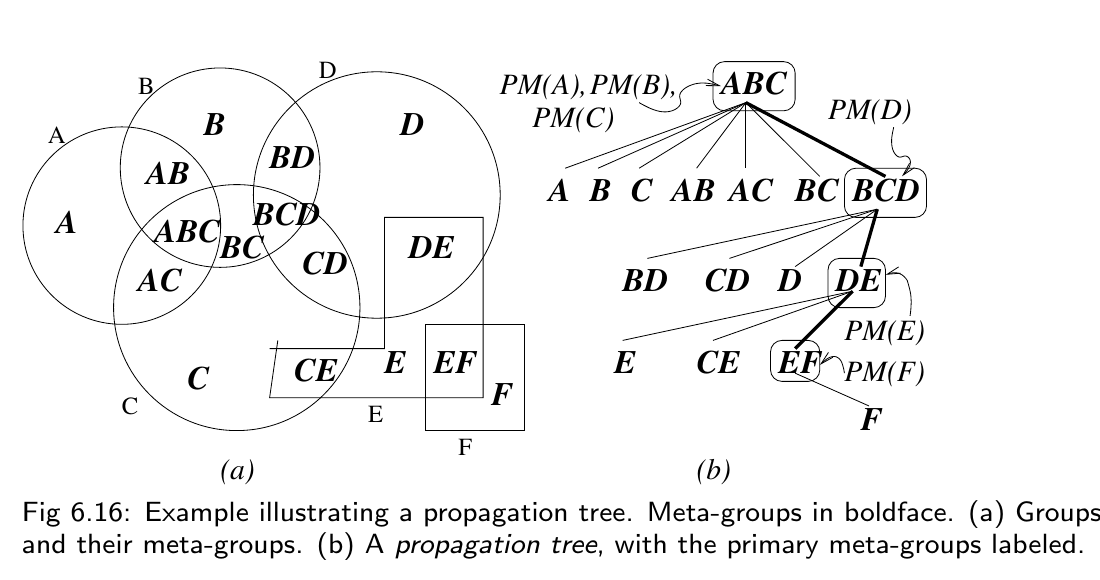
\includegraphics[trim=0 105 0 0,clip,width=.86\linewidth,height=.49\paperheight,keepaspectratio]{assets/week07-source-2025/propagation-tree-example-full.png}
\end{center}
\smallnote{左图把用户组的交集划分为 meta-group；右图把这些交集组织成传播树。粗体框为 primary meta-group，消息先到 $PM(G)$，再沿唯一子树路径下发。}
\end{frame}

\begin{frame}{Propagation Tree 的顺序逻辑}
\begin{itemize}
  \item 每个进程保存 $SV_i[k]$：自己发出的、将穿过 $PM(G_k)$ 的消息数；
  \item 每个 PM manager 保存 $RV_{manager}[k]$：已收到 $P_k$ 消息的数量；
  \item 只有 $SV_i[z]=RV_i[k]$ 时，PM(Gz) manager 才能处理来自 $P_k$ 的下一条消息；
  \item 非 primary meta-group 不直接接收 sender 消息，顺序已由上层 PM 确定；
  \item FIFO + 树路径唯一性共同保证下层成员看到的顺序。
\end{itemize}
\end{frame}

\begin{frame}{Propagation Tree：完整中文伪代码（发送端）}
\small
每个进程 $P_i$ 保存 $SV_i[1..h]$，其中 $h$ 是 primary meta-group 的数量。
当 $P_i$ 要向组 $G$ 组播消息 $M$ 时：
\begin{enumerate}
  \item 向 $PM(G)$ 的 manager 发送 $M(i,G,SV_i)$；
  \item 计算 $PMset$：该消息沿传播树必须经过的全部 primary meta-group；
  \item 对每个 $PM_x\in PMset$，执行 $SV_i[x]\leftarrow SV_i[x]+1$。
\end{enumerate}
\vfill
\callout{时间戳含义}{$SV_i[x]$ 不是“发给组 $x$ 的消息数”，而是 $P_i$ 已发送、且路径会穿过 primary meta-group $x$ 的消息数。它记录潜在因果前驱。}
\end{frame}

\begin{frame}{Propagation Tree：完整中文伪代码（manager）}
\scriptsize
primary manager $P_i$ 还保存 $RV_i[1..n]$。当 meta-group $MG$ 的 manager 从上层收到 $M(k,G,SV_k)$ 时：
\begin{enumerate}
  \item 若 $MG$ 是 primary meta-group，则缓冲消息，直到
  \[
  SV_k[i]=RV_i[k].
  \]
  条件表示：$P_k$ 先前所有必须经过本 PM 的消息都已处理。
  \item 条件满足后，令 $RV_i[k]\leftarrow RV_i[k]+1$。
  \item 对每个被 $MG$ 包含的 child meta-group，把同一 $M(k,G,SV_k)$ 发给 child manager。
  \item 若没有 child meta-group，则把消息交给当前 meta-group 内的每个进程。
\end{enumerate}
\smallnote{非 primary manager 无需执行向量等待；primary 层先确定顺序，FIFO 的父子链路再把该顺序逐层保留到叶子。}
\end{frame}

\begin{frame}{Propagation Tree：因果正确性四种情况}
\small
设 $M$ 发往 $G$，$M'$ 发往 $G'$，且某个进程同时属于 $G\cap G'$。
\begin{tabularx}{\linewidth}{>{\bfseries}p{1.4cm}p{3.2cm}X}
\toprule
情况 & 两个 primary meta-group 的位置 & 为什么交集成员仍按因果序交付 \\
\midrule
(a) & $PM(G)$ 是 $PM(G')$ 的祖先 & $M$ 先经过上层 PM；FIFO 保证 $M'$ 不能越过它。 \\
(b) & $PM(G')$ 是 $PM(G)$ 的祖先 & $M$ 的因果信息在共同路径上先被处理，再允许 $M'$ 下发。 \\
(c) & 两个 PM 位于同一分支 & 下层 PM 的向量等待条件阻止 $M'$ 提前。 \\
(d) & 两个 PM 在交集成员祖先路径上汇合 & 两条路径在共同祖先处形成统一的先后约束。 \\
\bottomrule
\end{tabularx}
\vfill
\callout{共同理由}{若两个组有交集，两个 PM 都必须是交集 meta-group 的祖先；向量等待确定 PM 层顺序，FIFO 再把顺序保持到叶子。}
\end{frame}

\begin{frame}{CO 与 Total Order 的实现风格}
\begin{tabularx}{\linewidth}{>{\bfseries}p{3cm}XX}
\toprule
风格 & 典型方法 & 关键顺序信息 \\
通信历史 & RST、KS、Lamport、NewTop & 向量、日志、因果摘要 \\
Privilege/token & Totem、on-demand & token 持有者按序分配 \\
Moving sequencer & Chang--Maxemchuck、Pinwheel & token 携带序号与待排序消息 \\
Fixed sequencer & propagation tree、ISIS、Amoeba & 固定中心或树层级排序 \\
Destination agreement & Lamport 三阶段、协议式 agreement & 目的地之间协商最终顺序 \\
\bottomrule
\end{tabularx}
\end{frame}

\sectionframe{十、故障容忍的组播语义}{组播不是原子的：一个节点交付了消息，并不自动说明其他正确/故障节点看到了什么。}

\begin{frame}{为什么要定义故障语义}
\begin{itemize}
  \item multicast 可能只到达部分目的地；
  \item sender、网络、接收进程都可能在不同时间失败；
  \item 恢复动作必须知道“谁已经交付、谁最终必须交付”；
  \item uniform 规格还把 faulty process 的 delivery 纳入约束；
  \item 没有统一语义，复制、回滚和重试会出现分叉。
\end{itemize}
\end{frame}

\begin{frame}{Uniform Reliable Multicast：Validity / Agreement / Integrity}
\begin{tabularx}{\linewidth}{>{\bfseries}p{2.6cm}X}
\toprule
Validity & 正确进程 multicast 的 $M$，所有正确进程最终 delivery $M$。 \\
Uniform Agreement & 任何正确或故障进程 delivery $M$，所有正确进程最终 delivery $M$。 \\
Uniform Integrity & 每个进程至多 delivery 一次，且只有 sender 曾 multicast 过 $M$ 才能 delivery。 \\
\bottomrule
\end{tabularx}
\vfill
\callout{差别}{Agreement 比 Validity 更强，因为它连“已经故障但曾经交付”的进程也纳入触发条件。}
\end{frame}

\begin{frame}{Uniform FIFO、Causal、Total Order 与 Timeliness}
\begin{itemize}
  \item FIFO：同一进程先 broadcast $M$ 再 broadcast $M'$，任何进程都不能先 delivery $M'$；
  \item CO：若 $M$ 因果先于 $M'$，则不能先 delivery $M'$；
  \item TO：任意两进程若都 delivery $M,M'$，顺序必须相同；
  \item Real-time timeliness：在真实时间 $t$ multicast 的消息，不能晚于 $t+\Delta$；
  \item Local-time timeliness：相对于每个进程自己的本地时钟给出上界。
\end{itemize}
\end{frame}

\sectionframe{十一、RPF 与 Steiner：把组播树放回网络成本中}{组播不仅要“顺序正确”，还要在链路数量、带宽、延迟和故障域之间做结构选择。}

\begin{frame}{Reverse Path Forwarding（RPF）}
\begin{itemize}
  \item 网络层组播利用拓扑信息；桥接 LAN 常用 spanning tree 学习目的地；
  \item IP 层 RPF 用“到源的下一跳”近似 rooted spanning tree，而不显式存储整棵树；
  \item 节点从正确的反向路径收到消息，才向其他链路转发；
  \item 其他入口的重复消息直接丢弃；
  \item 消息数更接近 $|N|$ 而不是 $|L|$。
\end{itemize}
\end{frame}

\begin{frame}{RPF：正确性直觉}
\begin{enumerate}
  \item 对源 $x$，每个节点选择一个 Next hop(x)；
  \item 消息从 $x$ 到达节点 $i$ 时，若入口邻居是 Next hop(x)，说明它沿着朝源的最短/估计路径反向到达；
  \item $i$ 向除入口外的所有链路转发；
  \item 从其他入口收到的副本不会再次转发，因此可以截断广播洪泛。
\end{enumerate}
\vfill
\callout{限制}{RPF 依赖路由表稳定；拓扑变化或路由环会造成丢包或重复，需要序号/TTL/修复机制。}
\end{frame}

\begin{frame}{Steiner tree：连接指定目的地而非所有节点}
\begin{itemize}
  \item 给定加权图 $G=(N,L)$ 与终端集合 $N'\subseteq N$；
  \item 找子图 $L'\subseteq L$，使 $(N',L')$ 连通；
  \item 允许使用不在 $N'$ 中的 Steiner points；
  \item 最小权 Steiner tree 是 NP-complete，需要近似/启发式；
  \item 网络成本为树边总成本，目的地成本为各终端路径成本之和。
\end{itemize}
\end{frame}

\begin{frame}{Kou--Markowsky--Berman（KMB）启发式}
\scriptsize
\begin{enumerate}
  \item 在终端集合 $N'$ 上构造 complete distance graph，边权为原图中的最短路长度；
  \item 在 distance graph 上求 MST $T'$；
  \item 将 $T'$ 的每条边展开成原图中的对应最短路径，得到 $G_s$；
  \item 在 $G_s$ 上再求 MST；
  \item 删除不必要边，使叶子尽量都为终端，得到 Steiner tree。
\end{enumerate}
\normalsize
\vfill
\callout{保证}{KMB 的近似比为 2；步骤 1 的最短路计算通常主导复杂度。}
\end{frame}

\begin{frame}{Delay-bounded Steiner tree：加入时延约束}
\begin{itemize}
  \item 每条边 $l$ 有成本 $C(l)$ 和整数延迟 $D(l)$；
  \item 给源 $s$、终端集合 $N'$ 和延迟上界 $\Delta$；
  \item 目标：最小化树边成本，同时满足任意终端 $v$：
\end{itemize}
\[
\sum_{l\in path(s,v)}D(l)<\Delta.
\]
\begin{itemize}
  \item 这是“低成本”与“低尾延迟”的联合优化；
  \item 在 GPU 集群中，延迟约束可替换为 step time 或 collective deadline。
\end{itemize}
\end{frame}

\begin{frame}{Constrained cheapest path 与闭包图}
\begin{itemize}
  \item 对任意终端对 $(x,y)$，计算满足 delay $<\Delta$ 的最低成本路径；
  \item 用动态规划求 $C_d(x,y)$：路径总延迟恰为 $d$；
  \item 取 $P_C(x,y)=\min_{d<\Delta}C_d(x,y)$；
  \item 在终端集合上构造 closure graph，再用贪心方法连接所有终端；
  \item 最后把闭包边展开回原图，删除展开产生的环。
\end{itemize}
\[
C_d(x,y)=\min_{z:(z,y)\in L}
\left\{C_{d-D(z,y)}(x,z)+C(z,y)\right\}.
\]
\smallnote{递推式枚举最后一条边 $(z,y)$；若 $d-D(z,y)<0$ 或子路径不可达，该候选成本视为无穷。}
\end{frame}

\begin{frame}{CSTCD 与 CSTC 两种启发式}
\begin{tabularx}{\linewidth}{>{\bfseries}p{2.6cm}X}
\toprule
CSTCD & 选择 $C(u,v)/(\Delta- PD(s,u)-D(u,v))$ 较小的边，同时考虑增量成本与剩余时延。 \\
CSTC & 只选择满足总时延约束的最低成本边，优先压低成本。 \\
\bottomrule
\end{tabularx}
\vfill
\callout{差异}{CSTCD 会主动为未来路径保留 delay slack；CSTC 更激进地压低当前成本，可能让后续可行边变少。}
\end{frame}

\begin{frame}{Delay-bounded Steiner 例子}
\begin{center}
\begin{tikzpicture}[x=1.65cm,y=1.25cm,>=Latex]
  \node[circle,draw=ADSBlue,fill=ADSBlue!10,minimum size=8mm] (s) at (0,1) {$s$};
  \node[circle,draw=ADSGray,fill=white,minimum size=8mm] (u) at (1.5,2) {$u$};
  \node[circle,draw=ADSOrange,fill=ADSOrange!12,minimum size=8mm] (a) at (3,2) {$a$};
  \node[circle,draw=ADSGray,fill=white,minimum size=8mm] (v) at (1.5,0) {$v$};
  \node[circle,draw=ADSOrange,fill=ADSOrange!12,minimum size=8mm] (b) at (3,0) {$b$};
  \draw[very thick,ADSGreen] (s)--node[above left]{(2,1)}(u);
  \draw[very thick,ADSGreen] (u)--node[above]{(3,2)}(a);
  \draw[very thick,ADSGreen] (s)--node[below left]{(2,1)}(v);
  \draw[very thick,ADSGreen] (v)--node[below]{(2,2)}(b);
  \draw[ADSGray,dashed] (u)--node[right]{(1,4)}(v);
  \node[anchor=west] at (3.7,1.55){\color{ADSBlue}$s$：源节点};
  \node[anchor=west] at (3.7,1.0){\color{ADSOrange}$a,b$：目的节点};
  \node[anchor=west] at (3.7,.45){\color{ADSGray}$u,v$：可选 Steiner 节点};
  \node[anchor=west] at (3.7,-.1){边标记为（成本，时延）};
\end{tikzpicture}
\end{center}
\smallnote{若 $\Delta=4$，两条源到目的路径的时延均为 3，满足约束；虚线边虽然成本低，但时延 4，会耗尽预算并可能使后续终端不可达。}
\end{frame}

\begin{frame}{复杂度与工程解释}
\begin{itemize}
  \item 约束最短路闭包计算主导，集中式代价约 $O(n^3)$；
  \item closure graph 上构造 $k$ 个终端的树约 $O(k^3)$；
  \item 将闭包边展开并去环约 $O(kn)$；
  \item 总体瓶颈仍是“在很多 delay budget 下找 cheapest path”；
  \item 工程上可按机架、可用区和链路等级分层近似，减少闭包规模。
\end{itemize}
\end{frame}

\sectionframe{十二、Core-based tree 与 AI 组播}{动态组成员不必从零建树：加入者向 core join，路径会逐渐 graft 成共享树。}

\begin{frame}{Core-based tree：按需长出来}
\begin{enumerate}
  \item 每个组选择一个或多个 core；
  \item 新 receiver 向 core 发送 unicast join；
  \item join 路径遇到 core 或已有树节点时，沿途边被 graft 到组播树；
  \item 树上节点用 core tree flooding 发送；
  \item 不在树上的 sender 先向 core 发送，碰到树后再沿树洪泛。
\end{enumerate}
\vfill
\callout{动态性}{成员变化只影响 join 路径附近；代价是 core 位置会造成路径不均衡和单点压力。}
\end{frame}

\begin{frame}{AI 基础设施映射：消息序的选择}
\begin{tabularx}{\linewidth}{>{\bfseries}p{2.8cm}XX}
\toprule
场景 & 推荐语义 & 原因 \\
参数/权重更新 & FIFO 或 CO & 同一源更新有顺序，跨源更新可并发 \\
配置与 schema & Total Order & 所有副本必须以相同顺序切换 \\
KV cache 失效 & CO + uniform agreement & 失效原因不能晚于新请求，故障节点也要收敛 \\
GPU collective & RPF/Steiner + deadline & 控制复制路径成本和尾延迟 \\
多租户订阅 & propagation tree & 共享 meta-group，避免每个组单独建树 \\
\bottomrule
\end{tabularx}
\end{frame}

\begin{frame}{课堂互动 1：给消息排序分层}
给出三条消息：$m_1$ 由 $P_1$ 发送，$P_2$ 收到后发送 $m_2$，$m_3$ 与二者无因果关系。
\begin{enumerate}
  \item 画出 $s(m_1)\prec s(m_2)$；
  \item 判断哪些 delivery 顺序违反 FIFO、CO、SYNC；
  \item 说明 $m_3$ 可以在哪些位置插入而不违反 CO；
  \item 若所有副本必须一致，为什么还要 total order？
\end{enumerate}
\end{frame}

\begin{frame}{课堂互动 2：寻找冠结构（crown）}
\begin{itemize}
  \item 给四个进程和四条 send/receive 对；
  \item 构造 $G_{\rightarrow}$，边条件为 $s\prec r'$；
  \item 找有向环并解释“谁在等待谁”；
  \item 改变一个 send 的本地先后，使图变为 DAG；
  \item 讨论改变后的执行是否仍满足 CO。
\end{itemize}
\end{frame}

\begin{frame}{课堂互动 3：RST 交付模拟}
\begin{enumerate}
  \item 给每个节点一个 $DELIV$ 向量；
  \item 让 $P_1$ 发送带 $ST$ 的消息给 $P_3$；
  \item 故意让一个因果前驱延迟，判断消息是否进入 buffer；
  \item 前驱到达后更新 $DELIV$，重新检查 delivery 条件；
  \item 估算 $n=8$ 时每条 RST 消息携带的元数据量。
\end{enumerate}
\end{frame}

\begin{frame}{课堂互动 4：中央 sequencer 与三阶段全序}
\begin{columns}[T,onlytextwidth]
\column{.47\textwidth}
\begin{enumerate}
  \item 两个 sender 并发发送 $m_1,m_2$；
  \item 中央 sequencer 按到达顺序编号；
  \item 比较 coordinator 故障时的恢复。
\end{enumerate}
\column{.47\textwidth}
\begin{enumerate}
  \item 每个节点提出 timestamp；
  \item 取最大 proposal；
  \item 解释为什么 temp\_Q 要等待 FINAL\_TS。
\end{enumerate}
\end{columns}
\end{frame}

\begin{frame}{课堂互动 5：GPU 组播树设计}
\begin{itemize}
  \item 给出 8 个 GPU、机架内/机架间 cost 与 delay；
  \item 先构造普通 Steiner tree，再加入 $\Delta$ 约束；
  \item 比较 CSTCD 与 CSTC 选出的边；
  \item 若某机架故障，RPF 和 core-based tree 如何恢复？
\end{itemize}
\end{frame}

\begin{frame}{本讲总结：从消息到组播树}
\begin{center}
\begin{tikzpicture}[node distance=7mm]
\nodebox{ADSBlue}{a}{A-execution};
\nodebox[right=of a]{ADSOrange}{fifo}{FIFO};
\nodebox[right=of fifo]{ADSGreen}{co}{CO};
\nodebox[right=of co]{ADSBlue}{rsc}{RSC / SYNC};
\nodebox[below=of co]{ADSOrange}{rst}{RST / KS};
\nodebox[right=of rst]{ADSGreen}{to}{Total Order};
\nodebox[right=of to]{ADSBlue}{tree}{Propagation / Steiner};
\draw[ADSBlue,\arrow] (a)--(fifo);
\draw[ADSOrange,\arrow] (fifo)--(co);
\draw[ADSGreen,\arrow] (co)--(rsc);
\draw[ADSBlue,\arrow] (co)--(rst);
\draw[ADSOrange,\arrow] (rst)--(to);
\draw[ADSGreen,\arrow] (to)--(tree);
\end{tikzpicture}
\end{center}
\vfill
\callout{带走一句话}{消息序不是越强越好；应选择刚好能支撑应用不变量的最弱语义，再用树、缓存和故障协议实现它。}
\end{frame}

\begin{frame}[plain]
\begin{tikzpicture}[remember picture,overlay]
  \fill[ADSBlue] (current page.north west) rectangle (current page.south east);
  \fill[ADSOrange] (current page.north west) rectangle ([yshift=-1.7mm]current page.north east);
  \node[align=center,text width=13cm] at (current page.center) {\fontsize{30}{38}\selectfont\color{white}\bfseries 先定义“何时能交付”\\[3mm]\large\color{white!80}再谈“如何把消息送给所有人”};
\end{tikzpicture}
\end{frame}

}

\long\def\partB{
\sectionframe{七、Optimal KS：只传播仍然必要的信息}{因果组播的难点不是“记录所有历史”，而是知道哪些历史信息已经可以安全删除。}

\begin{frame}{KS 的核心问题}
设 $M_{i,a}$ 是 $P_i$ 发出的第 $a$ 条 multicast。对目的地 $d$，记录“$d$ 是该消息目的地”直到：
\begin{enumerate}
  \item 已知 $M_{i,a}$ 已经交付给 $d$；
  \item 或已知某条消息已经在其因果未来发送给 $d$，传递性足以保证依赖。
\end{enumerate}
\vfill
\callout{最优性}{只要上述两个条件都未知，就必须保留并 piggyback 该目的地信息；任一条件确定后立即删除。}
\end{frame}

\begin{frame}{Propagation Constraint I / II}
\begin{columns}[T,onlytextwidth]
\column{.47\textwidth}
\blocktitle{Constraint I}
不知道 $M_{i,a}$ 是否已经被目的地 $d$ delivery。
\column{.47\textwidth}
\blocktitle{Constraint II}
不知道未来是否已发送一条给 $d$ 的消息，从而通过因果传递保证 $M_{i,a}$。
\end{columns}
\vfill
\begin{itemize}
  \item I、II 都为真：必须显式记录 $(source,timestamp,dest)$；
  \item I 为假：消息已交付，删除该目的地；
  \item II 为假：未来消息承担依赖，删除该目的地；
  \item 两者都为假：信息完全冗余。
\end{itemize}
\end{frame}

\begin{frame}{KS 的信息结构：显式与隐式跟踪}
\begin{itemize}
  \item 显式：LOG 和 outgoing metadata 中存放 $(source,ts,Dests)$；
  \item 隐式：已交付或一定会按 CO 交付的消息不再存储；
  \item 日志项的目的地集合变空时可删除；
  \item 对同一源的旧 timestamp，若新条目已覆盖，则旧条目也可通过集合逻辑清理；
  \item 这样元数据规模随“尚未被证明安全”的依赖增长，而不是随全部历史增长。
\end{itemize}
\end{frame}

\begin{frame}{KS 完整中文伪代码：发送端构造 $OM$}
\scriptsize
\begin{enumerate}
  \item $clock_j\leftarrow clock_j+1$。
  \item 对当前消息的每个目的地 $d$，令 $OM\leftarrow LOG_j$，逐项处理 $o=(s,t,D_o)$：
  \begin{itemize}\scriptsize
    \item 若 $d\notin D_o$：$D_o\leftarrow D_o\setminus Dests(M)$；
    \item 若 $d\in D_o$：$D_o\leftarrow(D_o\setminus Dests(M))\cup\{d\}$。
  \end{itemize}
  \item 若某条同源旧记录的目的地集合为空，且 $OM$ 中已有更新 timestamp，则删除旧记录。
  \item 向 $d$ 发送 $(j,clock_j,M,Dests(M),OM)$。
\end{enumerate}
\normalsize
\vfill
\callout{两种删除}{当前组播会替旧依赖向共同路径传播，但共同目的地 $d$ 仍必须保留，直到它验证并交付该因果前驱。}
\end{frame}

\begin{frame}{KS 完整中文伪代码：发送后更新 $LOG$}
\scriptsize
\begin{enumerate}
  \item 完成对所有目的地的发送后，对每个 $l\in LOG_j$：
  \[
  l.Dests\leftarrow l.Dests\setminus Dests(M).
  \]
  \item 执行 $PURGE\_NULL\_ENTRIES(LOG_j)$：若同源记录 $(s,t)$ 的目的地集合为空，且存在更新记录 $(s,t'),t'>t$，则删除旧记录。
  \item 把当前消息加入日志：
  \[
  LOG_j\leftarrow LOG_j\cup\{(j,clock_j,Dests(M))\}.
  \]
\end{enumerate}
\normalsize
\vfill
\callout{为何不立即删除所有空条目}{空集合仍可能承担“这个 timestamp 已出现”的知识；出现更新的同源记录后，旧信息才可由单调性隐式推断。}
\end{frame}

\begin{frame}{KS 完整中文伪代码：接收与交付}
\scriptsize
$P_j$ 从 $P_k$ 收到 $(k,t_k,M,Dests,OM)$：
\begin{enumerate}
  \item 对每条 $o=(m,t,D_o)\in OM$，若 $j\in D_o$，等待 $SR_j[m]\ge t$。
  \item 所有因果前驱满足后交付 $M$，并令 $SR_j[k]\leftarrow t_k$。
  \item $OM\leftarrow OM\cup\{(k,t_k,Dests)\}$。
  \item 对所有 $o\in OM$：$o.Dests\leftarrow o.Dests\setminus\{j\}$，因为 $j$ 已完成当前交付。
\end{enumerate}
\normalsize
\vfill
\callout{安全性}{只有元数据明确要求当前目的地等待的依赖才会阻塞；其他目的地的责任继续随消息传播。}
\end{frame}

\begin{frame}{KS 完整中文伪代码：合并与剪枝}
\scriptsize
将收到的 $OM$ 与本地 $LOG_j$ 按源进程分组：
\begin{enumerate}
  \item 收到记录较旧，且对应本地记录已被删除或已变为空：标记收到记录为冗余。
  \item 本地记录较旧，而更新收到记录已经蕴含其状态：标记本地旧记录为冗余。
  \item timestamp 相同的两条记录合并目的地责任，只保留仍未被证明安全的目的地。
  \item 删除所有已标记条目，把剩余 $OM$ 并入 $LOG_j$。
  \item 再执行 $PURGE\_NULL\_ENTRIES(LOG_j)$。
\end{enumerate}
\normalsize
\smallnote{剪枝只能删除“已交付”或“保证会按因果序交付”的信息；不能证明安全的依赖必须继续显式携带。}
\end{frame}

\begin{frame}{KS 信息剪枝图}
\begin{center}
\begin{tikzpicture}[x=2.1cm,y=1.15cm,>=Latex]
  \foreach \x/\lab in {0/$e_0$,1/$e_1$,2/$e_2$,3/$e_3$}
    \node[circle,draw=ADSBlue,fill=white,minimum size=7mm] (e\x) at (\x,0) {\lab};
  \draw[\arrow,ADSGray] (e0)--(e1);
  \draw[\arrow,ADSGray] (e1)--(e2);
  \draw[\arrow,ADSGray] (e2)--(e3);
  \nodebox[above=of e2,minimum width=2.2cm]{ADSGreen}{dest}{首次向 $d$ 发送};
  \draw[\arrow,ADSGreen] (e2)--(dest);
  \node[align=center,ADSOrange] at (0.5,-.75){必须显式携带\\“$d$ 尚需收到 $M$”};
  \node[align=center,ADSGreen] at (2.65,-.75){可由后续发送隐式保证\\旧目的地信息可剪枝};
\end{tikzpicture}
\end{center}
\smallnote{圆点是因果链上的事件。到达“首次向 $d$ 发送”的边界前，元数据必须显式说明 $d$ 的责任；越过边界后，新的消息已经承接该责任。}
\end{frame}

\begin{frame}{KS 的第二个剪枝视角}
\begin{center}
\begin{tikzpicture}[node distance=9mm and 15mm,>=Latex]
  \nodebox{ADSBlue}{src}{事件 $e$\\产生依赖};
  \nodebox[above right=of src]{ADSOrange}{a}{分支 A};
  \nodebox[below right=of src]{ADSOrange}{b}{分支 B};
  \nodebox[right=of a]{ADSGreen}{ad}{A 已向 $d$ 发送};
  \nodebox[right=of b]{ADSGray}{bn}{B 尚未向 $d$ 发送};
  \draw[\arrow,ADSGray] (src)--(a);
  \draw[\arrow,ADSGray] (src)--(b);
  \draw[\arrow,ADSGreen] (a)--(ad);
  \draw[\arrow,ADSGray] (b)--(bn);
  \node[ADSGreen,below=2mm of ad,align=center]{A 分支可删去\\$d$ 的旧责任};
  \node[ADSOrange,below=2mm of bn,align=center]{B 分支仍必须\\显式携带 $d$};
\end{tikzpicture}
\end{center}
\smallnote{剪枝按因果路径分别判断：某一分支已经把消息发给 $d$，不意味着其他分支也安全；只有所有相关路径的责任都被承接时才能彻底删除。}
\end{frame}

\begin{frame}{KS 例子：为什么元数据会沿因果边移动}
\begin{itemize}
  \item $P_5$ 的消息发给 $P_4,P_6$，其目的地信息进入后续消息的 piggyback；
  \item 当 $P_4$ 已知 $P_6$ 会沿因果路径收到依赖时，部分条目被删除；
  \item 同一条消息在不同进程的 LOG 中，目的地集合可能不同；
  \item 这不是不一致，而是各节点对“已交付/必交付”的知识不同。
\end{itemize}
\end{frame}

\begin{frame}{KS 例图：追踪一个 multicast 的 Dests}
\begin{center}
\begin{tikzpicture}[node distance=12mm and 20mm,>=Latex]
  \nodebox{ADSBlue}{p5}{$P_5$\\发送 $M$};
  \nodebox[above right=of p5]{ADSGreen}{p4}{$P_4$\\已交付 $M$};
  \nodebox[below right=of p5]{ADSOrange}{p6}{$P_6$\\尚未交付};
  \nodebox[right=of p4]{ADSBlue}{m2}{$P_4$ 发送后续消息 $M'$\\携带 $Dests=\{P_6\}$};
  \draw[\arrow,ADSGreen] (p5)--node[above left]{$M$}(p4);
  \draw[\arrow,ADSOrange] (p5)--node[below left]{$M$ 延迟}(p6);
  \draw[\arrow,ADSBlue] (p4)--(m2);
\end{tikzpicture}
\end{center}
\smallnote{$P_4$ 自己已交付，所以可从目的地集合中删除 $P_4$；但 $P_6$ 尚未交付，责任必须随 $M'$ 继续传播。课堂上继续追踪该条目何时能从 LOG 删除。}
\end{frame}

\sectionframe{八、Total Order：所有共同目的地看到同一顺序}{因果序只禁止颠倒原因和结果；全序还要把并发消息排成一个所有人相同的顺序。}

\begin{frame}{Total Order 的定义与动机}
\begin{itemize}
  \item 对任意两个同时交付 $M_x,M_y$ 的进程，交付顺序必须一致；
  \item 解决副本更新的 coherence：所有副本按同一顺序应用更新；
  \item 全序可以额外包含 causal order，也可以只要求一个共同排列；
  \item 代价是排序、确认或 sequencer，通常比 CO 更高。
\end{itemize}
\vfill
\callout{例子}{配置变更、模型版本切换、schema migration 和副本状态机都常用 total order。}
\end{frame}

\begin{frame}{中央 sequencer：最简单的全序}
\begin{enumerate}
  \item $P_i$ 把 multicast 请求发给 coordinator；
  \item coordinator 按到达顺序分配序号，并把消息发给组成员；
  \item 成员从 coordinator 的顺序 delivery；
  \item 时间约 2 次消息 hop，消息数约为每个目的地 1 次转发。
\end{enumerate}
\vfill
\callout{瓶颈}{coordinator 是吞吐、带宽和故障单点；因此需要移动 sequencer、固定 sequencer 或 destination agreement。}
\end{frame}

\begin{frame}{图例：total order 解决副本更新顺序}
\begin{center}
\begin{tikzpicture}[node distance=8mm and 16mm,>=Latex]
  \nodebox{ADSBlue}{s1}{$P_1$\\更新 $m_1$};
  \nodebox[below=of s1]{ADSBlue}{s2}{$P_2$\\更新 $m_2$};
  \nodebox[right=of $(s1)!0.5!(s2)$,minimum width=2.6cm]{ADSOrange}{seq}{Sequencer\\分配 10、11};
  \nodebox[above right=of seq]{ADSGreen}{r1}{副本 $R_1$\\10:$m_2$，11:$m_1$};
  \nodebox[right=of seq]{ADSGreen}{r2}{副本 $R_2$\\10:$m_2$，11:$m_1$};
  \nodebox[below right=of seq]{ADSGreen}{r3}{副本 $R_3$\\10:$m_2$，11:$m_1$};
  \draw[\arrow,ADSGray] (s1)--(seq);
  \draw[\arrow,ADSGray] (s2)--(seq);
  \draw[\arrow,ADSOrange] (seq)--(r1);
  \draw[\arrow,ADSOrange] (seq)--(r2);
  \draw[\arrow,ADSOrange] (seq)--(r3);
\end{tikzpicture}
\end{center}
\smallnote{网络到达次序可以不同，但副本必须按 sequencer 给出的序号交付。图中所有副本都先应用 $m_2$，再应用 $m_1$。}
\end{frame}

\begin{frame}{三阶段全序：消息与队列状态}
\begin{tabularx}{\linewidth}{>{\ttfamily\bfseries}p{3.6cm}X}
\toprule
REVISE\_TS & 发送者提出初始 Lamport timestamp，消息进入 temp\_Q 但不可交付 \\
PROPOSED\_TS & 每个进程返回自己的 proposed timestamp \\
FINAL\_TS & 发送者取所有 proposal 的最大值，宣布最终 timestamp \\
\bottomrule
\end{tabularx}
\vfill
\begin{itemize}
  \item temp\_Q 按 timestamp 排序；
  \item 只有队首且 deliverable 的消息才移动到 delivery\_Q；
  \item FINAL\_TS 让所有节点最终使用相同排序键。
\end{itemize}
\end{frame}

\begin{frame}{三阶段全序：为什么需要“先暂存、后交付”}
\begin{enumerate}
  \item REVISE\_TS 到达时，其他节点还不知道最终 timestamp；
  \item 若立即交付，后来可能出现更小 timestamp 的消息，顺序无法回退；
  \item 因此先放入 temp\_Q，标记 undeliverable；
  \item 收到 FINAL\_TS 后重新排序；
  \item 队首变为 deliverable 时，才按序移动到 delivery\_Q。
\end{enumerate}
\end{frame}

\begin{frame}{Total Order 完整例子：两个并发更新如何统一}
\small
$P_1,P_2$ 并发发送 $m_1,m_2$；中央 sequencer 按收到顺序编号，先看到 $m_2$。
\begin{center}
\begin{tabularx}{.96\linewidth}{>{\bfseries}p{1.4cm}>{\raggedright\arraybackslash}p{3.8cm}>{\raggedright\arraybackslash}X}
\toprule
步骤 & sequencer / 网络事件 & 副本队列与交付 \\
\midrule
1 & sequencer 收到 $m_2$，分配序号 10 & $P_3$ 收到 $(10,m_2)$，可暂存但等待更早序号。 \\
2 & sequencer 收到 $m_1$，分配序号 11 & $P_3$ 先收到 $(11,m_1)$，不能越过序号 10。 \\
3 & $P_3$ 收到 $(10,m_2)$ & 队列按序号排列为 $(10,m_2),(11,m_1)$。 \\
4 & 交付队列出队 & $P_3$ 按 $m_2\rightarrow m_1$ 交付；其他副本使用相同序号得到相同顺序。 \\
\bottomrule
\end{tabularx}
\end{center}
\callout{注意}{全序解决的是“所有副本相同”，不保证顺序符合发送者主观的真实时间；这里的权威顺序来自 sequencer。}
\end{frame}

\begin{frame}{三阶段全序：完整中文伪代码（发起者）}
\scriptsize
状态：$clock$、$priority$；队列项包含 $M,tag,sender,timestamp,deliverable$。
\begin{enumerate}
  \item $P_i$ 要组播 $(M,tag)$：$clock\leftarrow clock+1$，向所有进程发送 \texttt{REVISE\_TS(M,i,tag,clock)}。
  \item 等待每个 $P_j$ 的 \texttt{PROPOSED\_TS(j,i,tag,ts$_j$)}。
  \item $finalTs\leftarrow\max_j ts_j$，向所有进程发送 \texttt{FINAL\_TS(i,tag,finalTs)}。
  \item $clock\leftarrow\max(clock,finalTs)$。
\end{enumerate}
\normalsize
\vfill
\callout{为何取最大 proposal}{任何目的地已经观察到的优先级都不能被最终时间戳倒退，否则不同节点可能形成不同相对顺序。}
\end{frame}

\begin{frame}{三阶段全序：完整中文伪代码（接收者）}
\scriptsize
\begin{enumerate}
  \item 收到 \texttt{REVISE\_TS(M,j,tag,clk)}：
  \begin{itemize}\scriptsize
    \item $priority\leftarrow\max(priority+1,clk)$；
    \item 向 $temp\_Q$ 插入 $(M,tag,j,priority,false)$；
    \item 回复 \texttt{PROPOSED\_TS(i,j,tag,priority)}。
  \end{itemize}
  \item 收到 \texttt{FINAL\_TS(j,tag,clk)}：找到对应队列项，设 $deliverable=true$，更新时间戳并重排 $temp\_Q$。
  \item 若该项位于队首，将其移入 $delivery\_Q$；随后连续移动所有“位于队首且可交付”的项。
  \item 从 $delivery\_Q$ 交付 $(M,tag,j,ts)$ 时，$clock\leftarrow\max(clock,ts)+1$。
\end{enumerate}
\normalsize
\smallnote{实现还需用 $(timestamp,sender,tag)$ 等确定性复合键打破最终时间戳平局。}
\end{frame}

\begin{frame}{Total order 例子与复杂度}
\begin{tabularx}{\linewidth}{>{\bfseries}p{2.2cm}XX}
\toprule
阶段 & 网络动作 & 队列状态 \\
\midrule
提出 & 发送者广播 \texttt{REVISE\_TS} & 各节点插入不可交付的临时项 \\
协商 & 目的地返回 \texttt{PROPOSED\_TS} & 发送者取所有 proposal 的最大值 \\
确定 & 广播 \texttt{FINAL\_TS} & 各节点重排；只有队首且 deliverable 才交付 \\
\bottomrule
\end{tabularx}
\vfill
\begin{itemize}
  \item 延迟：约 3 个消息 hop；
  \item 每次组播：请求广播、proposal 汇聚、final 广播；
  \item 队列空间取决于并发但尚未确定最终时间戳的消息数。
\end{itemize}
\end{frame}


}

\long\def\partC{
\sectionframe{四、顺序层级与程序模拟}{顺序越强，越容易验证；顺序越弱，并发越高，但实现者要维护更多因果信息。}

\begin{frame}{消息顺序的包含关系}
\begin{center}
\begin{tikzpicture}[node distance=6mm,>=Latex]
  \nodebox[minimum width=2.35cm]{ADSGreen}{rsc}{RSC / SYNC\\同步握手可调度};
  \nodebox[right=of rsc,minimum width=2.35cm]{ADSOrange}{co}{CO\\因果关系不重排};
  \nodebox[right=of co,minimum width=2.35cm]{ADSBlue}{fifo}{FIFO\\同一发送者不重排};
  \nodebox[right=of fifo,minimum width=2.35cm]{ADSGray}{aa}{A\\任意异步执行};
  \draw[\arrow,ADSGreen] (rsc)--node[above]{包含于}(co);
  \draw[\arrow,ADSOrange] (co)--node[above]{包含于}(fifo);
  \draw[\arrow,ADSBlue] (fifo)--node[above]{包含于}(aa);
\end{tikzpicture}
\end{center}
\vspace{-2mm}
\[
RSC\subseteq CO\subseteq FIFO\subseteq A.
\]
\begin{itemize}
  \item A 的并发度最高，验证最难；
  \item SYNC/RSC 的顺序限制最强，程序最容易推理；
  \item CO 是常见折中：保留因果语义，同时允许无因果消息并发。
\end{itemize}
\end{frame}

\begin{frame}{一个“强语义—高并发”决策表}
\begin{tabularx}{\linewidth}{>{\bfseries}p{2.4cm}XXX}
\toprule
语义 & 保证什么 & 代价 & 典型用途 \\
\midrule
A & 只保证无因果环 & 最低控制开销，最难验证 & 高吞吐 best-effort \\
FIFO & 同一发送者顺序 & 序列号与缓存 & 单源日志、流式更新 \\
CO & 因果链不颠倒 & vector/依赖摘要 & 配置、协作、缓存失效 \\
SYNC/RSC & 握手与更强全局顺序 & 阻塞、可能死锁 & 小规模强协调协议 \\
\bottomrule
\end{tabularx}
\end{frame}

\begin{frame}{在同步系统上模拟异步程序}
\begin{itemize}
  \item 若执行是 RSC，按 non-separated linear extension 安排事件；
  \item 把相邻的 send/receive 作为一个同步原子动作；
  \item 原异步偏序保持不变，只改变具体时间轴；
  \item 若执行非 RSC，可把每条信道建模为控制进程 $P_{i,j}$，让 sender 与 receiver 解耦；
  \item 代价：额外控制进程和消息，且实现更复杂。
\end{itemize}
\end{frame}

\begin{frame}{在异步系统上模拟同步程序}
\begin{itemize}
  \item 按同步程序的偏序调度事件；
  \item 当同步 send 被调度时，等待对端 ACK 后才算 send 完成；
  \item 每条通信因此引入一次握手延迟；
  \item 若程序包含非确定性 receive，还要决定先匹配哪个发送者；
  \item 这就引出二元会合与无冠结构调度（crown-free scheduling）。
\end{itemize}
\end{frame}

\begin{frame}{同步程序在异步 runtime 上的调度难点}
\begin{enumerate}
  \item 多个 send/receive 在同一节点同时 enabled；
  \item 选择不同的匹配顺序可能产生不同偏序；
  \item 不能只“看到消息就处理”，还要避免跨进程循环等待；
  \item 调度器需要同时满足安全性（无冠结构）与进展性（最终能配对）；
  \item 还要兼顾 fairness 和控制消息开销。
\end{enumerate}
\end{frame}

\sectionframe{五、二元会合}{在异步系统中实现同步 send：用优先级打破对称等待。}

\begin{frame}{Bagrodia 算法的假设}
\begin{itemize}
  \item receive 始终 enabled；
  \item send 一旦 enabled 就持续 enabled；
  \item 用 PID/优先级引入非对称性；
  \item 每个进程一次只调度一个 send；
  \item 消息类型：$M$、$ack(M)$、$request(M)$、$permission(M)$。
\end{itemize}
\end{frame}

\begin{frame}{优先级规则：谁阻塞，谁先让路}
\begin{columns}[T,onlytextwidth]
\column{.47\textwidth}
\blocktitle{情况 A：高优先级 $\rightarrow$ 低优先级}
\begin{center}
\begin{tikzpicture}[node distance=13mm,>=Latex]
  \nodebox{ADSBlue}{hi1}{高优先级};
  \nodebox[right=of hi1]{ADSOrange}{lo1}{低优先级};
  \draw[\arrow,ADSBlue] (hi1.north east) to[bend left=16] node[above]{$M$} (lo1.north west);
  \draw[\arrow,ADSGreen] (lo1.south west) to[bend left=16] node[below]{$ack(M)$} (hi1.south east);
\end{tikzpicture}
\end{center}
直接发送 $M$，发送方阻塞到 ACK 返回。
\column{.47\textwidth}
\blocktitle{情况 B：低优先级 $\rightarrow$ 高优先级}
\begin{center}
\begin{tikzpicture}[node distance=13mm,>=Latex]
  \nodebox{ADSOrange}{lo2}{低优先级};
  \nodebox[right=of lo2]{ADSBlue}{hi2}{高优先级};
  \draw[\arrow,ADSOrange] (lo2.north east) to[bend left=20] node[above]{$request(M)$} (hi2.north west);
  \draw[\arrow,ADSGreen] (hi2.south west) to[bend left=20] node[below]{$permission(M)$} (lo2.south east);
\end{tikzpicture}
\end{center}
先申请许可，获准后再发送真正的 $M$。
\end{columns}
\vfill
\callout{避免成环}{阻塞依赖被优先级定向：高优先级可以等待 ACK，低优先级必须先取得许可。}
\end{frame}

\begin{frame}{Bagrodia：低优先级发送给高优先级}
\begin{enumerate}
  \item $P_i$ 向更高优先级 $P_j$ 发送 $request(M)$；
  \item 等待期间仍可处理来自更高优先级的 $M'$，并返回 $ack(M')$；
  \item 若收到更低优先级的 request，则发送 permission 并等待对应 $M'$；
  \item 收到 permission(M) 后，$P_i$ 才执行真正的 send(M)；
  \item 这样每次阻塞都沿优先级方向，不形成冠结构。
\end{enumerate}
\end{frame}

\begin{frame}{Bagrodia：高优先级发送给低优先级}
\begin{enumerate}
  \item 直接执行 send(M)；
  \item 发送方阻塞，直到收到 $ack(M)$；
  \item 阻塞期间，来自更高优先级的消息和来自更低优先级的 request 进入队列；
  \item 收到 ACK 后 send event 完成，再按队列顺序处理挂起消息。
\end{enumerate}
\vfill
\callout{直觉}{高优先级“占用通道”，低优先级先取得许可；优先级把可能的环压成一条链。}
\end{frame}

\begin{frame}{Bagrodia：完整中文事件处理规则}
\scriptsize
\begin{enumerate}
  \item SEND 到低优先级：send(M)，阻塞至 ack(M)；
  \item SEND 到高优先级：send(request(M))，等待 permission(M)，期间处理高优先级消息；
  \item 收到低优先级 request：回 permission，并等待其消息 M；
  \item 收到高优先级 M：执行 RECEIVE(M)，回 ack(M)；
  \item 解阻塞后，从队列取下一条消息并按上述规则处理。
\end{enumerate}
\normalsize
\end{frame}

\sectionframe{六、组通信与因果交付}{组播把一个点到点顺序问题扩展成“多个目的地必须看到哪些共同顺序”。}

\begin{frame}{Unicast、multicast、broadcast}
\begin{columns}[T,onlytextwidth]
\column{.47\textwidth}
\begin{itemize}
  \item unicast：一个发送者、一个目的地；
  \item multicast：发送给任意进程子集；
  \item broadcast：发送给系统或组内所有节点。
\end{itemize}
\column{.47\textwidth}
\begin{itemize}
  \item 网络层硬件 multicast 难以提供应用指定的顺序；
  \item 组成员关系可能动态变化；
  \item 不同应用需要不同故障容忍语义；
  \item 因此顺序和可靠性通常在应用层 overlay 实现。
\end{itemize}
\end{columns}
\end{frame}

\begin{frame}{开放组与闭合组}
\begin{itemize}
  \item closed group：发送者属于目的组；
  \item open group：发送者可以不在目的组中；
  \item 开放组下 source--destination 关系有四类：SSSG、MSSG、SSMG、MSMG；
  \item 组的数量理论上可达 $O(2^n)$，不能为每个组都维护一棵独立树；
  \item 需要共享结构，例如 meta-group 和 propagation tree。
\end{itemize}
\end{frame}

\begin{frame}{图例：四类 multicast 关系}
\begin{tabularx}{\linewidth}{>{\bfseries}p{1.7cm}XX}
\toprule
类型 & 发送关系 & 常见实现思路 \\
\midrule
SSSG & 一个源 $\rightarrow$ 一个组 & 单棵源树或直接广播 \\
MSSG & 多个源 $\rightarrow$ 一个组 & 共享 sequencer、token 或目的地协商 \\
SSMG & 一个源 $\rightarrow$ 多个组 & 复用前缀路径，在分叉处复制 \\
MSMG & 多个源 $\rightarrow$ 多个组 & meta-group、传播树与分层顺序控制 \\
\bottomrule
\end{tabularx}
\vfill
\smallnote{分类中的“多个组”允许组之间重叠；重叠成员正是跨组因果顺序最难处理的位置。}
\end{frame}

\begin{frame}{组播为什么会破坏顺序}
\begin{center}
\begin{tikzpicture}[node distance=9mm and 18mm,>=Latex]
  \nodebox{ADSBlue}{a}{$P_1$\\先发 $m_1$};
  \nodebox[below=of a]{ADSOrange}{b}{$P_2$\\收到后发 $m_2$};
  \nodebox[above right=of a]{ADSGreen}{r1}{副本 $R_1$\\先到 $m_1$};
  \nodebox[below right=of b]{ADSGreen}{r2}{副本 $R_2$\\先到 $m_2$};
  \draw[\arrow,ADSBlue] (a)--node[left]{$m_1$}(b);
  \draw[\arrow,ADSBlue] (a)--node[above]{$m_1$ 快}(r1);
  \draw[\arrow,ADSBlue,dashed] (a)--node[above,sloped]{$m_1$ 慢}(r2);
  \draw[\arrow,ADSOrange,dashed] (b)--node[below,sloped]{$m_2$ 慢}(r1);
  \draw[\arrow,ADSOrange] (b)--node[below]{$m_2$ 快}(r2);
\end{tikzpicture}
\end{center}
\smallnote{$m_1\prec m_2$，但链路延迟使 $R_2$ 先收到 $m_2$。因果组播必须在 $R_2$ 缓冲 $m_2$，直到 $m_1$ 可交付。}
\end{frame}

\begin{frame}{RST：用发送/交付矩阵表达因果依赖}
\begin{block}{状态}
$SENT[i,j]$：进程 $P_i$ 已向 $P_j$ 发送的消息数；$DELIV[k]$：本地已交付的 $P_k$ 消息数。
\end{block}
\begin{itemize}
  \item 每条消息携带发送者的 $SENT$ 摘要；
  \item 到达 $P_i$ 后，只有当对所有 $x$ 都有 $DELIV[x]\ge ST[x,i]$ 才能 delivery；
  \item delivery 后更新本地 $DELIV$，并合并收到的发送计数。
\end{itemize}
\end{frame}

\begin{frame}{RST 的交付条件：先满足原因，再处理结果}
\[
\forall x,\quad DELIV[x]\ge ST[x,i]
\quad\Longrightarrow\quad deliver(M).
\]
\begin{enumerate}
  \item $ST[x,i]$ 表示发送者认为目的地 $i$ 应已看到的第 $x$ 个消息；
  \item 若本地 $DELIV[x]$ 不足，说明存在因果前驱尚未交付；
  \item 消息进入 buffer，直到所有前驱满足；
  \item 无故障且传播时间有限时，条件最终满足，保证 liveness。
\end{enumerate}
\end{frame}

\begin{frame}{RST：完整中文伪代码}
\scriptsize
本地状态：$SENT[1..n,1..n]$ 初值为 0；$DELIV[1..n]$ 初值为 0。
\begin{block}{发送：$P_i$ 向 $P_j$ 发送应用消息 $M$}
1. 发送 $(M,SENT)$ 给 $P_j$；\\
2. $SENT[i,j]\leftarrow SENT[i,j]+1$。
\end{block}
\begin{block}{接收：$P_i$ 从 $P_j$ 收到 $(M,ST)$}
1. 缓冲 $M$，直到 $\forall x:\ DELIV[x]\ge ST[x,i]$；\\
2. 交付 $M$；\\
3. 对所有 $x,y$：$SENT[x,y]\leftarrow\max(SENT[x,y],ST[x,y])$；\\
4. $DELIV[j]\leftarrow DELIV[j]+1$；随后重新检查缓冲消息。
\end{block}
\normalsize
\smallnote{发送计数的递增顺序与消息携带的是“发送前摘要”相配套；若实现采用先递增再携带，交付条件也要一致修改。}
\end{frame}

\begin{frame}{RST 完整例子：向量条件如何阻塞消息}
\small
两个发送者的计数向量按 $[P_1,P_2]$ 记录；$P_2$ 在收到 $a$ 后发送 $b$。
\begin{center}
\begin{tabularx}{.96\linewidth}{>{\bfseries}p{1.3cm}>{\raggedright\arraybackslash}p{3.5cm}>{\raggedright\arraybackslash}X}
\toprule
步骤 & 状态/消息 & $P_3$ 的动作 \\
\midrule
1 & $P_1$ 发送 $a$，$ST(a)=[1,0]$ & $a$ 延迟；$DELIV_3=[0,0]$。 \\
2 & $P_2$ 收到 $a$ 后发送 $b$，$ST(b)=[1,1]$ & $b$ 先到，但检查 $DELIV_3[1]=0<1$，放入 buffer。 \\
3 & $a$ 到达 $P_3$ & delivery $a$，更新 $DELIV_3=[1,0]$。 \\
4 & 重新检查 $b$ & $DELIV_3\ge[1,1]$ 后 delivery $b$，更新为 $[1,1]$。 \\
\bottomrule
\end{tabularx}
\end{center}
\smallnote{向量摘要把“为什么 $b$ 不能先交付”变成可计算的条件，而不是依赖人工追踪整条因果链。}
\end{frame}

\begin{frame}{RST 的成本与适用边界}
\begin{tabularx}{\linewidth}{>{\bfseries}p{3.3cm}X}
\toprule
正确性 & FIFO channels + 交付条件，保证 causal safety \\
空间 & 每节点约 $n^2$ 个整数，每条消息也携带 $n^2$ 摘要 \\
时间 & 每次 send/receive 处理约 $O(n^2)$ \\
全广播简化 & 若所有消息广播，矩阵可压缩为更规则的向量/计数 \\
\bottomrule
\end{tabularx}
\vfill
\callout{工程权衡}{RST 直观但元数据很大；大规模 AI 服务通常使用稀疏依赖、分层向量或 epoch 摘要。}
\end{frame}


\begin{frame}{学习目标}
\begin{enumerate}
  \item 区分 arrival、receive、delivery 以及 FIFO、CO、SYNC 的语义；
  \item 用因果偏序解释消息为何会被 overtaken；
  \item 识别 RSC 执行和 crown，并解释同步 send 的死锁来源；
  \item 掌握 RST 因果交付、KS 信息裁剪和三阶段全序；
  \item 读懂 meta-group/propagation tree，并比较 RPF、Steiner 和 core-based tree；
  \item 为 AI 权重、配置、KV cache 选择合适的组播顺序与故障承诺。
\end{enumerate}
\vfill
\callout{核心问题}{系统真正需要的是“所有消息都按同一顺序到达”，还是“因果上不应颠倒的消息不被颠倒”？}
\end{frame}

\begin{frame}{本讲逻辑路线}
\begin{center}
\begin{tikzpicture}[node distance=8mm]
\nodebox{ADSBlue}{events}{事件偏序};
\nodebox[right=of events]{ADSOrange}{orders}{FIFO / CO / SYNC};
\nodebox[right=of orders]{ADSGreen}{delivery}{可交付条件};
\nodebox[right=of delivery]{ADSBlue}{groups}{组播与全序};
\nodebox[right=of groups]{ADSOrange}{faults}{故障与树};
\draw[ADSBlue,\arrow] (events)--(orders);
\draw[ADSOrange,\arrow] (orders)--(delivery);
\draw[ADSGreen,\arrow] (delivery)--(groups);
\draw[ADSBlue,\arrow] (groups)--(faults);
\end{tikzpicture}
\end{center}
\vfill
\callout{听课提示}{后面每一种算法都只是这条路线上的一个“实现点”，不是孤立的代码。}
\end{frame}

}

\long\def\partD{
\sectionframe{一、消息事件与顺序层级}{先把“发送、到达、交付”拆开，再讨论不同通信模型允许哪些事件偏序。}

\begin{frame}{记号：网络、事件与消息}
\begin{itemize}
  \item 网络 $N,L$，事件集合 $E$，因果关系记作 $\prec$；
  \item 消息 $M$ 的发送事件 $s(M)$、接收/到达事件 $r(M)$；
  \item $a\sim b$：事件 $a,b$ 在同一进程发生；
  \item $T=\{(s,r)\in E\times E\mid s\text{ 与 }r\text{ 是同一消息的发送/接收}\}$；
  \item 本讲将“消息到达 OS buffer”与“应用 delivery”明确区分。
\end{itemize}
\vfill
\callout{为什么要拆开}{消息可能已经到达，但由于因果依赖尚未满足，仍不能交付给应用。}
\end{frame}

\begin{frame}{Arrival、receive、delivery：同一消息的三个时刻}
\begin{center}
\begin{tikzpicture}[node distance=8mm]
\nodebox{ADSBlue}{send}{send(M)};
\nodebox[right=of send]{ADSOrange}{arrive}{到达缓冲区};
\nodebox[right=of arrive]{ADSGreen}{wait}{等待依赖};
\nodebox[right=of wait]{ADSBlue}{deliver}{delivery(M)};
\draw[ADSBlue,\arrow] (send)--(arrive);
\draw[ADSOrange,\arrow] (arrive)--(wait);
\draw[ADSGreen,\arrow] (wait)--(deliver);
\end{tikzpicture}
\end{center}
\vfill
\begin{itemize}
  \item FIFO 主要约束同一逻辑链路上的 delivery 顺序；
  \item CO 还要追踪不同发送者之间的因果链；
  \item 全序要求所有共同目的地对消息有相同 delivery 顺序。
\end{itemize}
\end{frame}

\begin{frame}{A-execution 与 FIFO execution}
\begin{columns}[T,onlytextwidth]
\column{.46\textwidth}
\begin{block}{A-execution}
事件因果关系是偏序，没有因果环；逻辑信道不保证 FIFO，例如无连接 IPv4。
\end{block}
\column{.49\textwidth}
\begin{block}{FIFO execution}
若同一发送者先发送 $M_1$ 再发送 $M_2$，同一接收者不能先交付 $M_2$。
\end{block}
\end{columns}
\vfill
\begin{itemize}
  \item 物理链路可能 FIFO，但逻辑 overlay 的多跳路径不一定 FIFO；
  \item 在非 FIFO 链路上可用 $\langle seq\_num,conn\_id\rangle$ 与接收缓存重建 FIFO。
\end{itemize}
\end{frame}

\begin{frame}{图例：A-execution 可以 FIFO，也可以非 FIFO}
\begin{center}
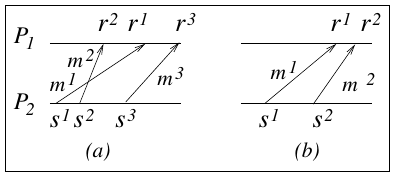
\includegraphics[width=.78\linewidth,height=.48\paperheight,keepaspectratio]{assets/week07-source-2025/async-fifo-execution-full.png}
\end{center}
\smallnote{左图中 $m^1$、$m^2$ 的交付顺序保持；右图中同一发送者的后发消息先到达，说明 A-execution 本身不提供 FIFO。}
\end{frame}

\begin{frame}{从链路 FIFO 到因果序：为什么还不够}
\begin{itemize}
  \item $P_1$ 先发送 $m_1$ 给 $P_2$；$P_2$ 收到后再发送 $m_2$ 给 $P_3$；
  \item 即使 $m_1$ 与 $m_2$ 走不同链路，$m_2$ 也不能在 $m_1$ 前被共同目的地处理；
  \item 这种“通过进程接力形成的先后”不是单条链路 FIFO 能表达的；
  \item 需要把 send 事件之间的因果关系传播到 delivery 条件中。
\end{itemize}
\vfill
\callout{过渡}{FIFO 只看同一发送者；causal order（CO）看整个 happens-before 链。}
\end{frame}

\sectionframe{二、Causal Order：让因果链不被颠倒}{CO 不要求无因果关系的消息排序，只禁止把“原因”放在“结果”之后。}

\begin{frame}{Causal Order 的定义}
对任意两对发送/接收事件 $(s,r),(s',r')\in T$，若 $r\sim r'$ 且 $s\prec s'$，则必须有 $r\prec r'$。
\[
(r\sim r'\ \land\ s\prec s')\Rightarrow r\prec r'.
\]
\begin{itemize}
  \item 发送事件有因果关系时，共同目的地必须按同样顺序 delivery；
  \item 若两个 send 事件并无因果关系，CO 对它们不施加顺序；
  \item 因而 CO 比全序更有并发度，比 FIFO 表达能力更强。
\end{itemize}
\end{frame}

\begin{frame}{CO 的四个时间线例子}
\begin{center}
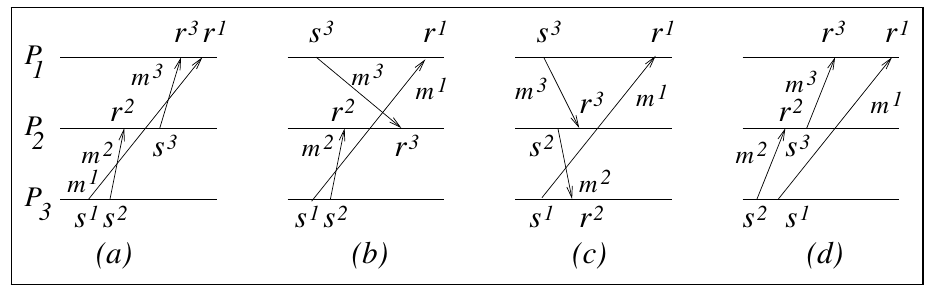
\includegraphics[width=.82\linewidth,height=.50\paperheight,keepaspectratio]{assets/week07-source-2025/causal-order-examples-full.png}
\end{center}
\smallnote{左侧例子违反 CO：$s^1\prec s^3$，却有 $r^3\prec r^1$；其余例子满足 CO，尤其是无因果关系时可以有不同交付顺序。}
\end{frame}

\begin{frame}{CO 的实现视角：arrival 不等于 delivery}
\begin{enumerate}
  \item 消息 $m$ 到达 OS buffer；
  \item 检查所有在 $send(m)$ 之前因果发生、且发给同一目的地的消息是否已经到达；
  \item 若存在 overtaken message，先缓存 $m$；
  \item 依赖满足后，才产生应用层 delivery 事件。
\end{enumerate}
\vfill
\callout{典型用途}{共享数据更新、分布式共享内存、公平资源分配、协作应用、事件通知和虚拟环境。}
\end{frame}

\begin{frame}{FIFO 完整例子：到达顺序不等于交付顺序}
\small
$P_1$ 依次发送 $m_1,m_2$ 给 $P_3$；$P_2$ 发送与它们无因果关系的 $x$。
\begin{center}
\begin{tabularx}{.96\linewidth}{>{\bfseries}p{1.5cm}>{\raggedright\arraybackslash}p{3.1cm}>{\raggedright\arraybackslash}X}
\toprule
时刻 & 到达 $P_3$ 的消息 & FIFO 接收/交付动作 \\
\midrule
$t_1$ & $m_2$ 先到（假设底层非 FIFO） & 不能交付，放入 buffer；$m_1$ 仍未到。 \\
$t_2$ & $x$ 到达 & $x$ 与 $P_1$ 的消息无关，可以直接 delivery。 \\
$t_3$ & $m_1$ 到达 & 先 delivery $m_1$，再释放 buffer 中的 $m_2$。 \\
\bottomrule
\end{tabularx}
\end{center}
\callout{结论}{FIFO 只约束同一发送者的消息：$m_1\prec m_2$；它不要求无关的 $x$ 必须排在二者之后。}
\end{frame}

\begin{frame}{因果序完整例子：结果不能跑到原因前面}
\small
$P_1$ 把更新 $u$ multicast 给 $P_2,P_3$；$P_2$ 收到 $u$ 后再 multicast $v$ 给 $P_3$。$w$ 与这条链并发。
\begin{center}
\begin{tabularx}{.96\linewidth}{>{\bfseries}p{1.2cm}>{\raggedright\arraybackslash}p{3.3cm}>{\raggedright\arraybackslash}X}
\toprule
步骤 & 事件 & $P_3$ 的处理 \\
\midrule
1 & $P_1\rightarrow\{P_2,P_3\}:u$ & $P_3$ 尚未收到 $u$。 \\
2 & $P_2$ 收到 $u$，发送 $v$ & 形成因果链 $u\prec v$。 \\
3 & $P_3$ 先收到 $v$ & 检查发现 $u$ 未 delivery，$v$ 进入 buffer。 \\
4 & $P_3$ 收到 $u$ & 先 delivery $u$，再 delivery 已满足依赖的 $v$；$w$ 可在两者之间交付。 \\
\bottomrule
\end{tabularx}
\end{center}
\smallnote{CO 不强迫 $w$ 与 $u,v$ 排序；它只禁止 $v$ 越过自己的因果前驱 $u$。}
\end{frame}

\begin{frame}{CO 退化为 FIFO 的条件}
\begin{itemize}
  \item 若 $m_1,m_2$ 由同一进程发送，则 $s(m_1)\prec s(m_2)$；
  \item 对同一目的地，CO 强制 $delivery(m_1)\prec delivery(m_2)$；
  \item 因此同一发送者到同一目的地时，CO 至少包含 FIFO；
  \item 对不同发送者，只有在存在因果链时才约束顺序。
\end{itemize}
\end{frame}

\begin{frame}{CO 的三个等价刻画}
\begin{tabularx}{\linewidth}{>{\bfseries}p{3.2cm}X}
\toprule
Message Order (MO) & 消息不能被同一因果链 overtaken；若 $s\prec s'$，则不允许 $r'\prec r$。 \\
Empty Interval (EI) & 对每个 $(s,r)\in T$，偏序中 $s$ 与 $r$ 之间的开区间为空。 \\
Common past/future & 消息的 send/receive 对之间不存在会破坏共同过去或共同未来的事件。 \\
\bottomrule
\end{tabularx}
\vfill
\callout{解释}{EI 把 CO 画成时空图：每条消息都可以在某个线性扩展中画成“垂直箭头”。}
\end{frame}

\begin{frame}{CO 不等于同一张时空图中的所有竖直箭头}
\begin{itemize}
  \item CO 要求“对每条消息，存在一个合适的线性扩展”；
  \item 不要求所有消息同时在同一个线性扩展中都没有中间事件；
  \item 如果所有消息都能在同一张图里画成竖直箭头，系统已经接近 synchronous execution；
  \item 这一区别解释了 CO 与 SYNC 之间仍存在大量并发空间。
\end{itemize}
\end{frame}

\sectionframe{三、同步执行、RSC 与 crown}{同步通信把 send/receive 绑定成握手，但任意异步执行不一定能在这种原语下重放。}

\begin{frame}{Synchronous execution：消息握手}
\begin{center}
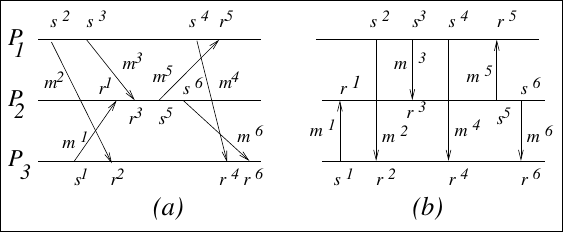
\includegraphics[width=.82\linewidth,height=.52\paperheight,keepaspectratio]{assets/week07-source-2025/synchronous-execution-full.png}
\end{center}
\smallnote{同步通信把发送和接收视为原子握手：$s(M)$ 与 $r(M)$ 具有相同 scalar timestamp，不允许 send 已完成而 receive 尚未配对。}
\end{frame}

\begin{frame}{同步因果关系 $\prec_s$}
同步因果关系是满足以下条件的最小传递关系：
\begin{enumerate}
  \item 同一进程中先发生的事件先于后发生事件；
  \item 若 $(s,r)\in T$，则任一事件 $x$ 在 $s$ 之前当且仅当它在 $r$ 之前，$s$ 在 $x$ 之前当且仅当 $r$ 在 $x$ 之前；
  \item 关系满足传递性。
\end{enumerate}
\vfill
\callout{timestamp}{存在标量映射 $T:E\rightarrow\mathbb{T}$，使得同一消息的 send/receive 时间戳相等，进程内事件严格递增。}
\end{frame}

\begin{frame}{异步程序使用同步原语：会发生什么？}
\begin{columns}[T,onlytextwidth]
\column{.47\textwidth}
\begin{itemize}
  \item $P_i$ 先 SEND 给 $P_j$；
  \item $P_j$ 同时先 SEND 给 $P_i$；
  \item 两个进程都在等待对方 RECEIVE；
  \item 同步 send 需要握手才能完成。
\end{itemize}
\column{.47\textwidth}
\begin{tikzpicture}[scale=.86,transform shape,x=1cm,y=.8cm,>=Latex]
  \draw[very thick,ADSBlue] (0,3.5)--(0,0) node[below]{$P_i$};
  \draw[very thick,ADSOrange] (4,3.5)--(4,0) node[below]{$P_j$};
  \fill[ADSBlue] (0,3) circle (2.2pt) node[left]{发送给 $P_j$};
  \fill[ADSOrange] (4,3) circle (2.2pt) node[right]{发送给 $P_i$};
  \draw[\arrow,ADSBlue] (0,3)--node[above,sloped]{$m_i$}(4,2.1);
  \draw[\arrow,ADSOrange] (4,3)--node[above,sloped]{$m_j$}(0,2.1);
  \node[draw=ADSOrange,rounded corners,align=center] at (2,.9){双方都等待对应接收\\没有进程能执行下一步};
\end{tikzpicture}
\end{columns}
\vfill
\callout{结论}{程序在异步消息模型中可执行，不代表它在同步通信原语下也可执行。}
\end{frame}

\begin{frame}{RSC execution：定义}
\begin{block}{Non-separated linear extension}
偏序 $(E,\prec)$ 的一个全序扩展，使每一对 $(s,r)\in T$ 之间没有其他事件落在开区间中。
\end{block}
\begin{itemize}
  \item 若异步执行存在这样的扩展，就称为 RSC（realizable with synchronous communication）；
  \item 直接枚举所有线性扩展是指数级的；
  \item 需要一个局部可检验的结构来判断是否存在同步重放。
\end{itemize}
\end{frame}

\begin{frame}{冠结构（crown）：同步重放失败的最小环}
\begin{center}
\begin{tikzpicture}[node distance=10mm and 24mm,>=Latex]
  \nodebox[minimum width=2.5cm]{ADSBlue}{m1}{$m_1=(s_1,r_1)$};
  \nodebox[right=of m1,minimum width=2.5cm]{ADSOrange}{m2}{$m_2=(s_2,r_2)$};
  \nodebox[below=of $(m1)!0.5!(m2)$,minimum width=2.5cm]{ADSGreen}{m3}{$m_3=(s_3,r_3)$};
  \draw[\arrow,ADSBlue] (m1)--node[above]{$s_1\prec r_2$}(m2);
  \draw[\arrow,ADSOrange] (m2)--node[right]{$s_2\prec r_3$}(m3);
  \draw[\arrow,ADSGreen] (m3)--node[left]{$s_3\prec r_1$}(m1);
\end{tikzpicture}
\end{center}
\begin{block}{定义}
crown 是消息对序列 $\langle(s_i,r_i)\mid 0\le i<k\rangle$，满足
$s_0\prec r_1,s_1\prec r_2,\ldots,s_{k-2}\prec r_{k-1},s_{k-1}\prec r_0$。
\end{block}
\smallnote{上图是大小为 3 的 crown。箭头不是消息链路，而是“某次发送必须排在另一消息接收之前”的调度依赖。}
\end{frame}

\begin{frame}{为什么 crown 会导致死锁}
\begin{enumerate}
  \item 同步 send 必须与对应 receive 原子配对；
  \item crown 中每个 send 的完成依赖另一个 receive；
  \item 但下一个 receive 又依赖其对应 send 完成；
  \item 因果关系绕一圈回到起点，没有任何消息可以先执行；
  \item 因而 crown 是“无法安排第一步”的证据。
\end{enumerate}
\vfill
\callout{注意}{crown 中相邻的 send/receive 不必发生在同一进程；它表达的是跨进程的循环依赖。}
\end{frame}

\begin{frame}{冠结构对 RSC 的刻画}
\begin{itemize}
  \item crown 中 $s_i$ 与 $r_{i+1}$ 可以位于同一进程，也可以跨进程；
  \item 非 CO 执行一定包含 crown；
  \item 某些 CO 但非同步的执行也包含 crown；
  \item 冠结构中的环意味着消息不能被串行调度，因此不是 RSC。
\end{itemize}
\vfill
\begin{block}{冠结构判据}
一个异步执行能够用同步通信实现（即属于 RSC），当且仅当该执行不包含 crown。
\end{block}
\callout{不要混淆}{“满足因果序”仍可能不是 RSC；CO 约束交付顺序，而 RSC 还要求每个 send/receive 能被排成不可分割的同步握手。}
\end{frame}

\begin{frame}{冠结构测试：把消息变成图}
\begin{enumerate}
  \item 在消息集合 $T$ 上定义 $[s,r]\rightarrow[s',r']\iff s\prec r'$；
  \item 构造有向图 $G_{\rightarrow}=(T,\rightarrow)$；
  \item 若图中存在有向环，则对应执行含 crown；
  \item 无环时，可按拓扑序找到 non-separated linear extension；
  \item 测试复杂度为 $O(|E|)$（更准确地说与通信事件数线性相关）。
\end{enumerate}
\vfill
\callout{线性扩展}{crown test 把“检查所有调度”转化为“检查一个依赖图是否有环”。}
\end{frame}

\begin{frame}{图例：冠结构测试的关系图}
\begin{center}
\begin{tikzpicture}[node distance=15mm and 20mm,>=Latex]
  \nodebox[minimum width=2.6cm]{ADSBlue}{a}{$m_1=[s_1,r_1]$};
  \nodebox[right=of a,minimum width=2.6cm]{ADSOrange}{b}{$m_2=[s_2,r_2]$};
  \nodebox[below=of $(a)!0.5!(b)$,minimum width=2.6cm]{ADSGreen}{c}{$m_3=[s_3,r_3]$};
  \draw[\arrow,ADSBlue] (a)--node[above]{$s_1\prec r_2$}(b);
  \draw[\arrow,ADSOrange] (b)--node[right]{$s_2\prec r_3$}(c);
  \draw[\arrow,ADSGreen] (c)--node[left]{$s_3\prec r_1$}(a);
\end{tikzpicture}
\end{center}
\begin{enumerate}
  \item 每个顶点代表一条消息，而不是一个事件；
  \item 若 $s_i\prec r_j$，就在 $m_i\rightarrow m_j$ 之间连有向边；
  \item 图中的 $m_1\rightarrow m_2\rightarrow m_3\rightarrow m_1$ 是有向环，因此原执行含 crown，不能同步重放；
  \item 若依赖图无环，按拓扑序配对执行各条消息即可得到 RSC 调度。
\end{enumerate}
\end{frame}

\begin{frame}{RSC 的等价时间戳刻画}
执行 $(E,\prec)$ 属于 RSC，当且仅当存在标量时间戳映射 $T:E\rightarrow\mathbb{N}$，使得：
\begin{enumerate}
  \item 对每条消息 $M$，同步握手的两个事件具有相同时间戳：
  \[
  T(s(M))=T(r(M));
  \]
  \item 对不是同一消息握手的事件 $a,b$，若 $a\prec b$，则
  \[
  T(a)<T(b).
  \]
\end{enumerate}
\vfill
\callout{解释}{同一条消息的 send/receive 被压缩为一个同步步骤；其他因果关系必须严格增加。crown 会迫使时间戳沿环严格递增并回到起点，因此不可能赋值。}
\end{frame}

}

\partD
\partC
\partB
\partA
\begin{frame}{消息协议边界卡：同一个“收到”可能不是同一个事件}
\small
\begin{itemize}
  \item \key{arrival}：消息进入内核、网络栈或协议缓冲区；
  \item \key{receive}：协议状态机取出并处理消息；
  \item \key{delivery}：应用层真正观察到消息并改变状态；
  \item FIFO/因果/全序通常约束的是 delivery，不是网卡中断的物理到达顺序。
\end{itemize}
\vfill
\begin{columns}[T,onlytextwidth]
\column{.48\textwidth}
\blocktitle{可靠性前提}
\begin{itemize}
  \item RST/KS 的简化伪代码假设消息最终可交付、序号单调且重复可去重；
  \item 若允许丢失或重启，必须加入重传、持久化和 epoch。
\end{itemize}
\column{.48\textwidth}
\blocktitle{中心排序器故障}
\begin{itemize}
  \item sequencer 挂掉后不能简单“换一个进程继续编号”；
  \item 需要 epoch/任期、状态转移和重复消息判定，通常还需要共识或持久化日志。
\end{itemize}
\end{columns}
\vfill
\callout{判断题}{“消息已经到达”不等于“应用已经交付”，“交付顺序一致”也不等于“与墙上时钟顺序一致”。}
\end{frame}
\end{document}
